\section{Деплой приложения на Heroku} \label{pril:e}

Для регистрации в Heroku\footnote{\url{https://signup.heroku.com/login}} необходима только электронная почта (рис.~\ref{pic:heroku_reg}).
\begin{figure}[ht]
    \centering
	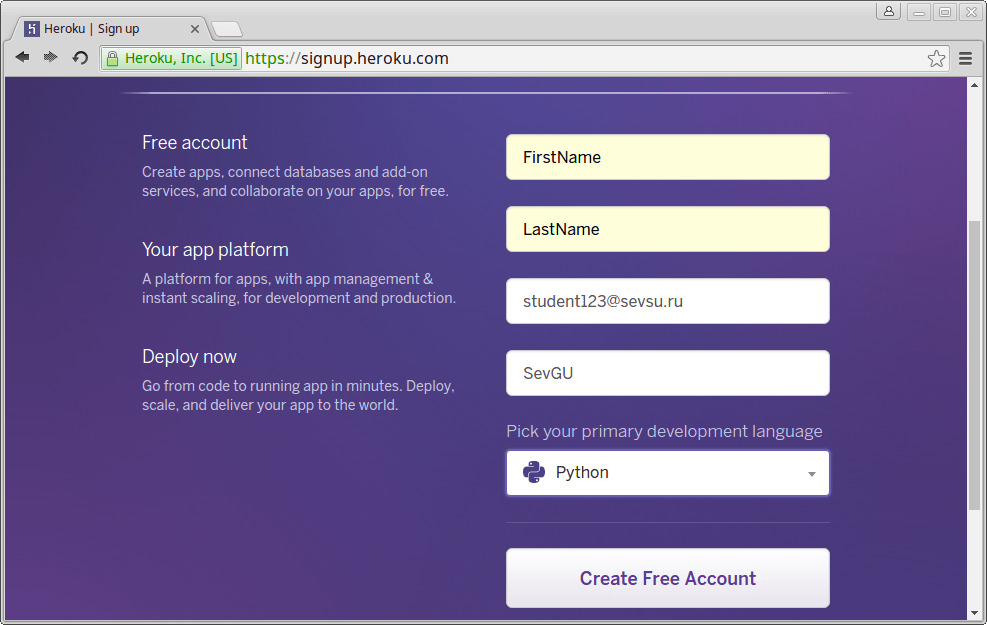
\includegraphics[width=\linewidth]{register}
    \caption{Регистрация в Heroku}\label{pic:heroku_reg}
\end{figure}

После регистрации, на указанный почтовый ящик приходит письмо с подтверждением регистрации, необходимо перейти по ссылке из письма и подтвердить регистрацию.

После подтверждения регистрации можно войти в свою учетную запись и ознакомиться с интерфейсом платформы.

Создадим новое приложение в разделе <<Personal Apps>> (рис.~\ref{pic:add_app}).
\begin{figure}[ht]
    \centering
	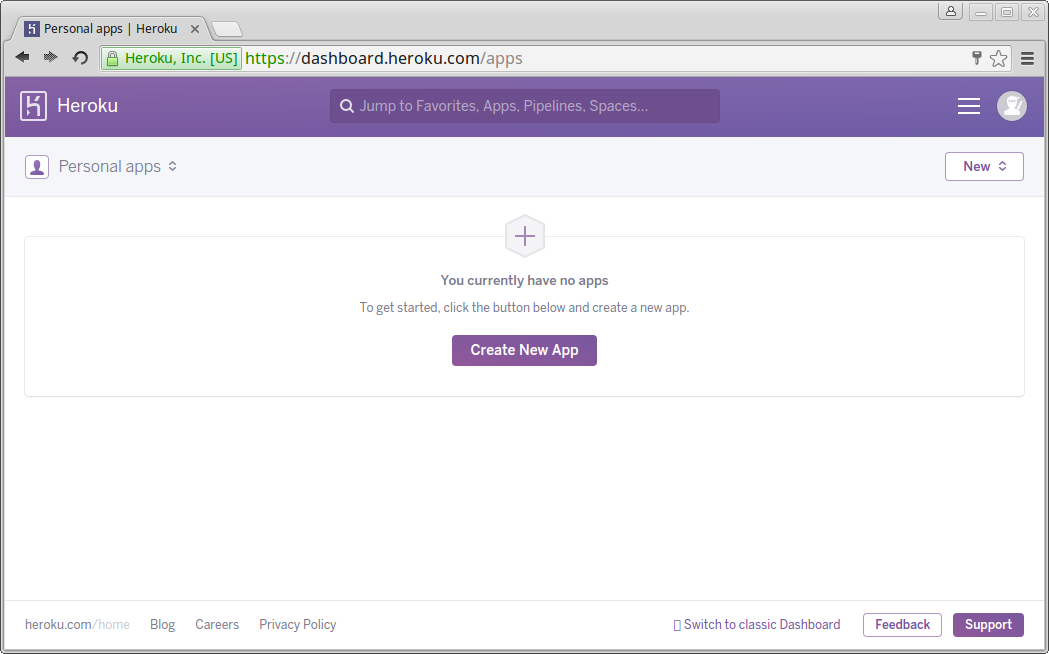
\includegraphics[width=0.7\linewidth]{createapp}
    \caption{Список созданных приложений в Heroku}\label{pic:add_app}
\end{figure}

Пусть имя приложения будет <<helloivt>> (рис.~\ref{pic:helloivt}).
\begin{figure}[ht]
    \centering
	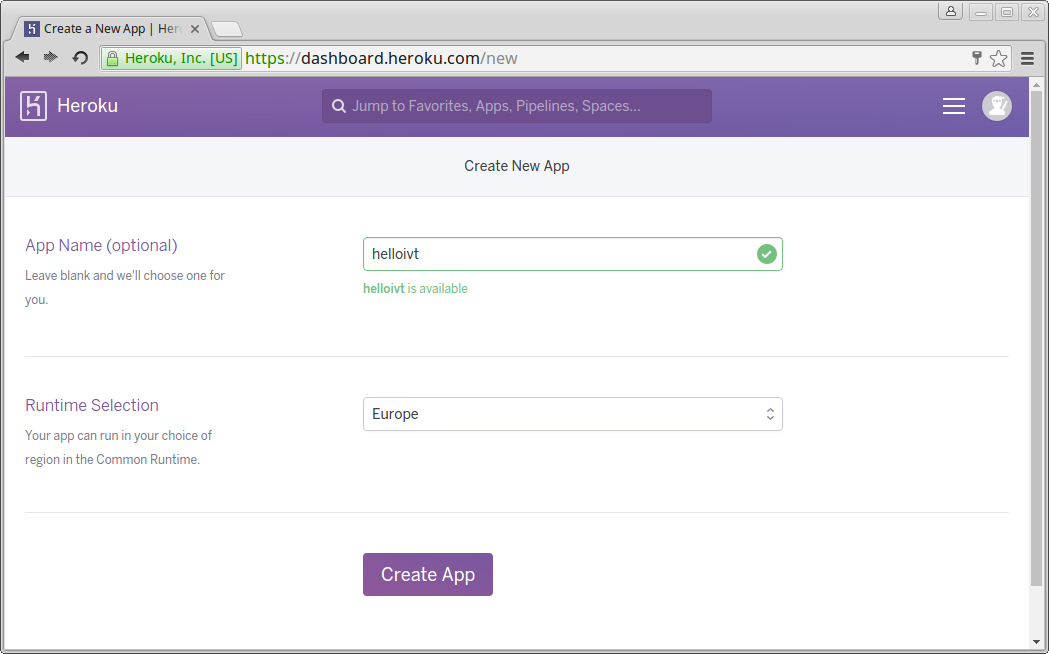
\includegraphics[width=\linewidth]{helloivt}
    \caption{Создание нового приложения}\label{pic:helloivt}
\end{figure}

Авторизуемся на сервере с Debian, устанавливаем heroku-cli и авторизуемся в Heroku:
\begin{lstlisting}
$ wget -O- https://toolbelt.heroku.com/install-ubuntu.sh | sh
$ heroku login
heroku-cli: Installing CLI... 21.83MB/21.83MB
Enter your Heroku credentials.
Email: student123@sevsu.ru
Password (typing will be hidden):
Logged in as student123@sevsu.ru
\end{lstlisting}

Добавляем контактные данные разработчика:
\begin{lstlisting}
$ git config --global --add user.email "student123@sevsu.ru"
$ git config --global --add user.name "Name Surname"
\end{lstlisting}

Клонируем репозиторий с тестовым приложением на Flask:
\begin{lstlisting}
$ git clone https://github.com/craigkerstiens/flask-helloworld
$ cd flask-helloworld/
\end{lstlisting}

Реиницилизируем репозиторий:
\begin{lstlisting}
$ git init
Reinitialized existing Git repository in /home/student/flask-helloworld/.git/
$ heroku git:remote -a helloivt
set git remote heroku to https://git.heroku.com/helloivt.git
\end{lstlisting}

Деплоим приложение в Heroku:
\begin{lstlisting}
$ git push heroku master
\end{lstlisting}

Переходим на страницу приложения\footnote{\url{https://helloivt.herokuapp.com/}, где <<helloivt>> "--- это имя приложения, заданное в веб-интерфейсе Heroku} и проверяем, страница должна выводить надпись <<Hello from Python!>> (рис.~\ref{pic:hellopy}).

\clearpage

\begin{figure}[ht]
    \centering
	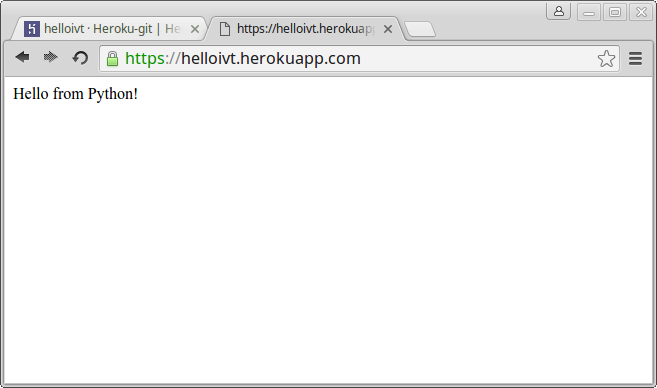
\includegraphics[width=\linewidth]{hello}
    \caption{Создание нового приложения}\label{pic:hellopy}
\end{figure}

Внесем изменения в приложение, отредактировав приветствие:
\begin{lstlisting}
$ nano app.py
    return "Hello from IVT student!"
$ git commit -am "First commit!"
[master 898f7d8] First commit!
 1 file changed, 1 insertion(+), 1 deletion(-)
$ git push heroku master
\end{lstlisting}

Обновляем страницу с приложением (рис.~\ref{pic:newhello}).
\begin{figure}[ht]
    \centering
	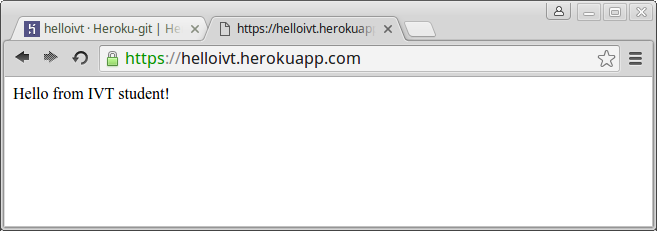
\includegraphics[width=\linewidth]{newhello}
    \caption{Изменения в приложении вступили в силу}\label{pic:newhello}
\end{figure}

\clearpage
